\documentclass{beamer}
\usetheme{metropolis}           % Use metropolis theme
\setbeamercovered{transparent}

\title{Miscellaneous topics}
\date{\today}
\author{Mine \c{C}etinkaya-Rundel}
\institute{Sta 771S - Teaching Statistics}

\begin{document}
\maketitle
 
 
% -------------------------------------------------------------------

\section{Teaching online}

% -------------------------------------------------------------------

\section{Fully online courses}

% -------------------------------------------------------------------

\begin{frame}
\frametitle{Various audiences}

\begin{itemize}

\item Small scale: university students

\item Large scale: massive open online course (MOOC)

\end{itemize}

\end{frame}

% -------------------------------------------------------------------

\begin{frame}
\frametitle{Synchronous vs. asynchronous}

\begin{itemize}

\item Synchronous: students "meet" with you online

\item Asynchronous: relies fully on previously recorded material

\item Hybrid: a bit of both

\end{itemize}

\end{frame}

% -------------------------------------------------------------------

\begin{frame}
\frametitle{Example: STA 104}

Hybrid course for a small university audience

\begin{itemize}

\item Online version of STA 101, offered in the summer, for credit, for Duke students

\item Virtual daily meetings on WebEx Training Center (recorded)

\item 90 mins / day, 5 days / week, lecture + lab

\item Breakout sessions for teamwork

\item Assignments and forums (Piazza) on Sakai

\item Materials posted on public course website

\end{itemize}

\end{frame}

% -------------------------------------------------------------------

\begin{frame}
\frametitle{STA 104 -- WebEx Training Center}

Recreating the classroom experience online

\begin{center}
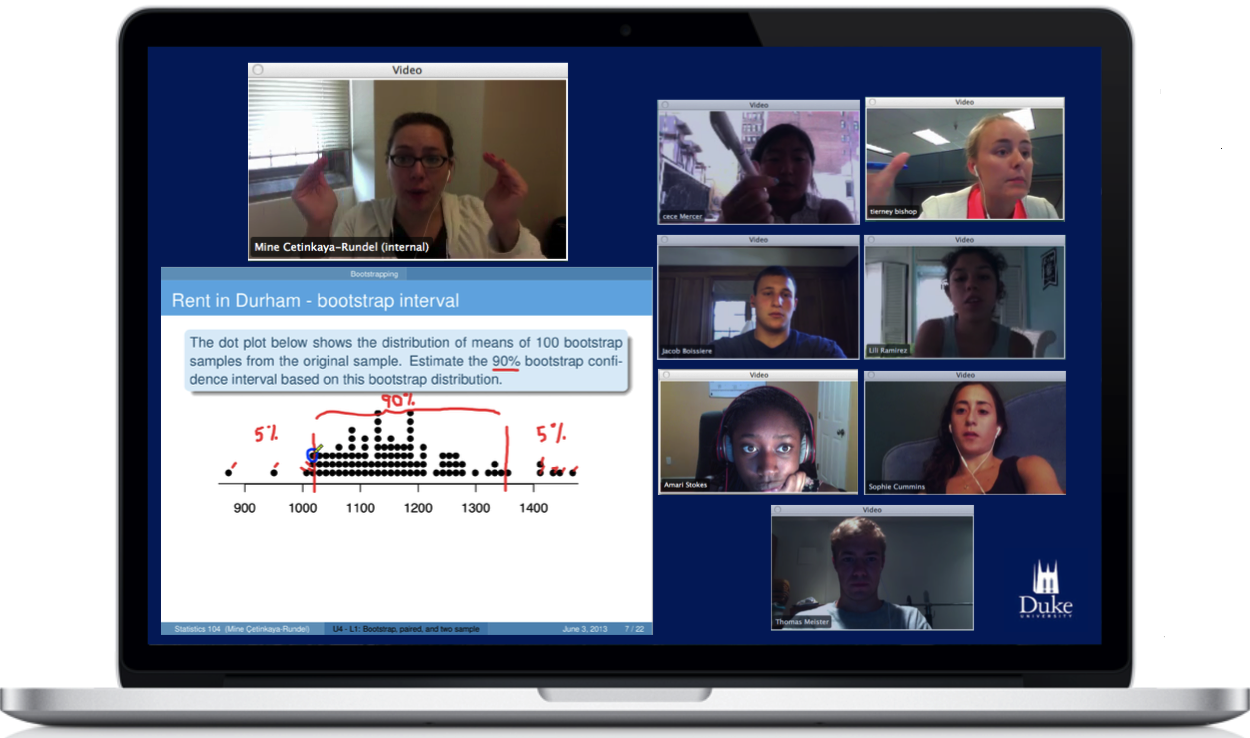
\includegraphics[width = \textwidth]{figures/sta104}
\end{center}

\end{frame}

% -------------------------------------------------------------------

\begin{frame}
\frametitle{STA 104 -- polling}

Recreating the clicker experience online

\begin{center}
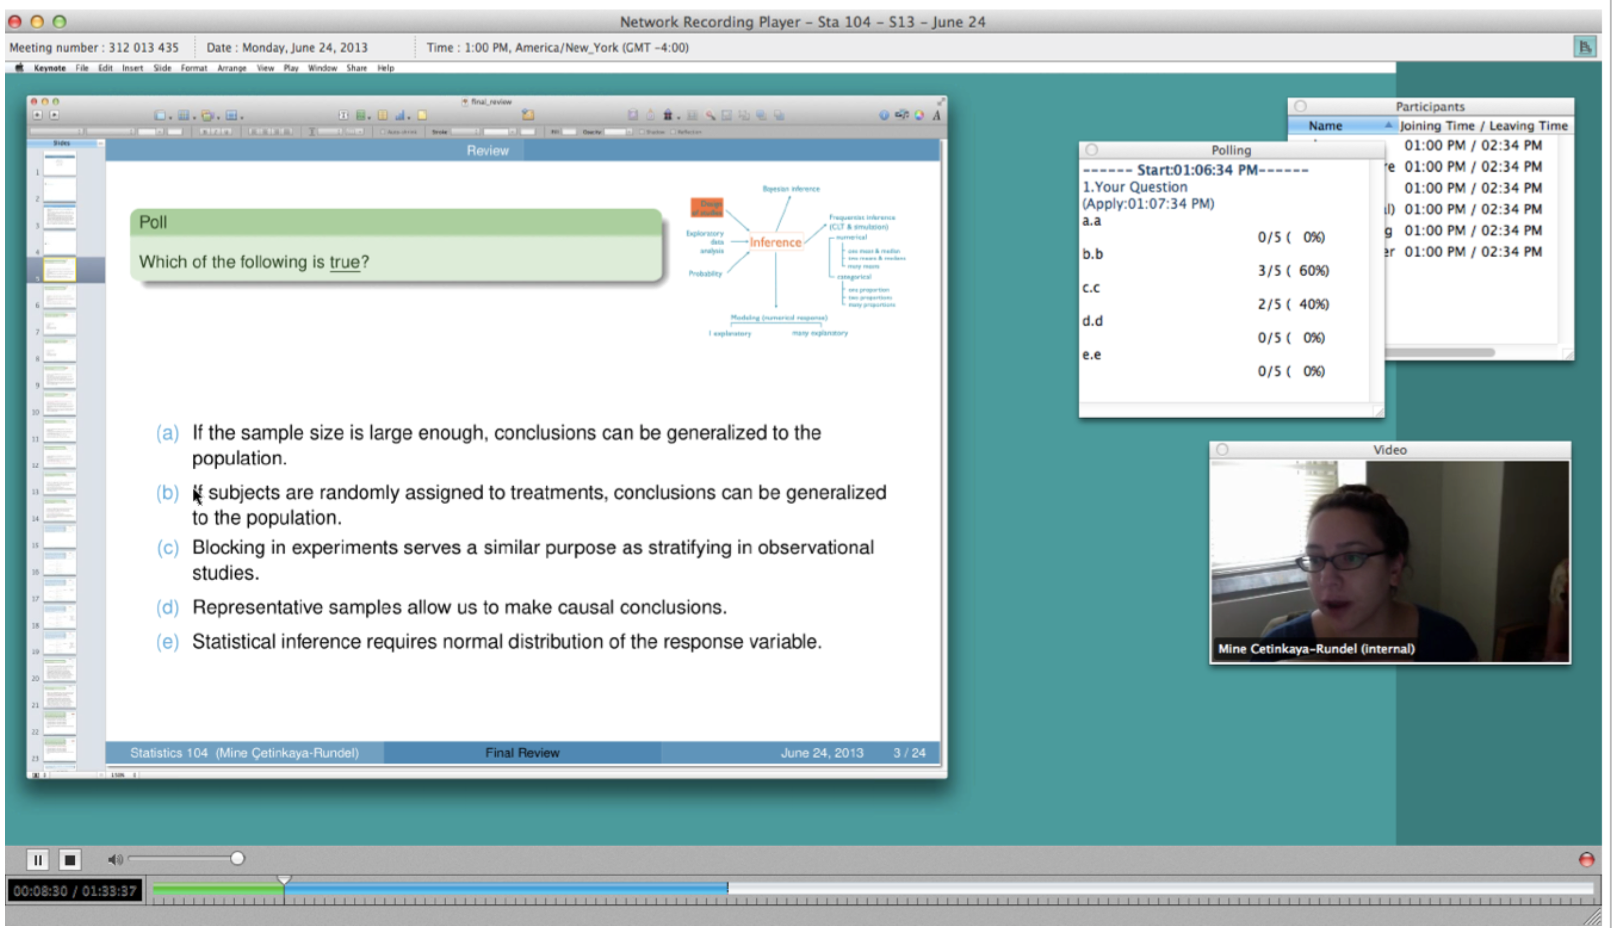
\includegraphics[width = \textwidth]{figures/polling}
\end{center}

\end{frame}

% -------------------------------------------------------------------

\begin{frame}
\frametitle{STA 104 -- student feedback}

\begin{itemize}

\item  ``I like the \textbf{convenience} of the online class but also the web chat structure makes it feel as if you are actually in a classroom. So it is the best of both worlds.�

\item ``I really enjoy the \textbf{videos}! They are a very helpful learning tool. It is also nice to have them to go back to at any time to clear up a concept.�

\item ``I like that the class is \textbf{discussion-based and interactive}. I enjoy working with my classmates on application exercises and we are able to explain concepts to each other in terms that we understand. I also like the various polls that we do during lectures because they \textbf{keep you engaged} and you can learn a lot from hearing other students explain the reasoning behind their answers.�

\end{itemize}

\end{frame}

% -------------------------------------------------------------------

\begin{frame}
\frametitle{STA 104 -- reflection}

Positive:
\begin{itemize}
\item Great experience
\item Synchronous sessions worthwhile
\item Assessment submission and grading on Sakai
\item Teams on Sakai for application activity submission and reveal
\item Performance assessments*
\end{itemize}
*Adopted in on-campus course \\

$\:$ \\

Questionable:
\begin{itemize}
\item Scalable
\item Exams on Sakai
\item One-on-one student support
\end{itemize}

\end{frame}

% -------------------------------------------------------------------

\begin{frame}
\frametitle{Example: MOOC}

\begin{itemize}

\item Data Analysis and Statistical Inference (DASI)

\item Now redesigned as the Statistics with R Specialization on Coursera
\begin{enumerate}
\item Introduction to Probability and Data
\item Inferential Statistics
\item Linear Regression and Modeling
\item Bayesian Statistics
\item Statistics Capstone Project
\end{enumerate}

\end{itemize}

\end{frame}

% -------------------------------------------------------------------

\begin{frame}
\frametitle{Preparing a MOOC}

It takes a village!

\begin{itemize}

\item Course design

\item Content and assessment generation

\item Video production

\item Backend support

\item Student support -- community TAs

\item ...

\end{itemize}

\end{frame}

% -------------------------------------------------------------------

\begin{frame}
\frametitle{MOOC: Assessments}

\begin{itemize}

\item Formative
\begin{itemize}
\item Suggested textbook exercises 
\item In-video questions
\end{itemize}

\item Summative
\begin{itemize}
\item Data analysis labs (R/RStudio or DataCamp)
\item Unit quizzes (10-15 MC questions, 2 attempts)
\item Exams
\item Data analysis project (peer assessment)
\end{itemize}

\end{itemize}

\end{frame}

% -------------------------------------------------------------------

\begin{frame}
\frametitle{MOOC: Why?}

\begin{itemize}

\item Making educational resources widely and freely* available

\item Good way to get your name out there

\item Resources can be re-used on campus as part of a hybrid course

\end{itemize}

\end{frame}

% -------------------------------------------------------------------

\section{Teaching with online resources}

% -------------------------------------------------------------------

\begin{frame}
\frametitle{Online resources}

Hybrid courses using

\begin{itemize}

\item Videos -- made by you vs. curated by you

\item Online quizzes -- immediate feedback

\item Online discussion forums

\end{itemize}

\end{frame}

% -------------------------------------------------------------------

\section{Assessment}

% -------------------------------------------------------------------

\begin{frame}
\frametitle{Levels of assessment}

\begin{itemize}

\item Course level

\item Program level

\end{itemize}

\end{frame}

% -------------------------------------------------------------------

\begin{frame}
\frametitle{How to assess}

\begin{itemize}

\item Set goals, e.g. at the end of this course/program students will be able to ...
\begin{itemize}
\item Use Guidelines for Assessment and Instruction in Statistics Education (GAISE) as a starting point
\end{itemize}

\item Collect data specifically addressing these goals, i.e. not just course grade information

\item Use widely used assessment scales, e.g. CAOS - Comprehensive Assessment of Outcomes in a First Statistics course

\item Do pre-post testing when possible
\begin{itemize}
\item Make it a part of the course so it doesn't feel like additional work for students
\end{itemize}

\end{itemize}

\end{frame}

% -------------------------------------------------------------------

\section{Course evaluations}

% -------------------------------------------------------------------

\begin{frame}
\frametitle{}

\begin{itemize}

\item Always do a mid-semester evaluation, and share summary of findings with students
\begin{itemize}
\item Encourage them to be constructive and specific
\item Address concerns explicitly
\item See if anything can be changed about the course in a way that doesn't negatively impact your course plan but also satisfies the students
\end{itemize}

\pause

\item Encourage students to provide feedback via the official course evaluation mechanism
\begin{itemize}
\item Set aside class time
\item Send reminders
\item Encourage them to be constructive and specific
\end{itemize}

\pause

\item Publicly available evaluations
\begin{itemize}
\item Remind yourself that voluntary response bias exists
\item Do not say (or write in an email) anything that you don't want posted publicly
\item Grow a thick skin :)
\end{itemize}

\end{itemize}

\end{frame}

% -------------------------------------------------------------------

\end{document}